\documentclass[a4paper]{article}
\usepackage{graphicx}
\usepackage{float} 
\usepackage{standalone}
\usepackage{adjustbox}
\usepackage{longtable} 
\usepackage{booktabs} 
\usepackage{rotating} 
\usepackage{datetime}
\usepackage{float}
\usepackage{fontawesome} % Paquete para íconos
\usepackage{amsmath}
\usepackage{enumitem}
\setlength{\parindent}{0pt} 
\graphicspath{{C:/Users/USER/Documents/econometria/tarea3/plot/}}
\usepackage[letterpaper]{geometry}

%opening
\title{Problem Set 3}
\author{Tannya Mainato \and Alan Del Rosario \and Mariuxi Gualán}
\date{\the\year-\twodigit\month-\twodigit\day}

\begin{document}

\maketitle


\section*{Mario Party}

Te gusta jugar Mario Party con tus amigos. En este juego, los jugadores deben recolectar estrellas para ganar. Las estrellas se encuentran en casillas especiales y, para desplazarse por el tablero, los jugadores
lanzan un dado con seis caras numeradas del 1 al 6. A ti te encanta ganar y te molestas mucho si pierdes.
Estás cerca de la victoria, así que comienzas a calcular tus probabilidades de coronarte campeón.

\begin{enumerate}[label=\alph*.]
	\item Es tu turno y vas a lanzar el dado. Necesitas sacar un 5 en el próximo lanzamiento para obtener la estrella. ¿Cuál es la probabilidad de que obtengas un 5?
		\begin{figure}[H]
			\centering
			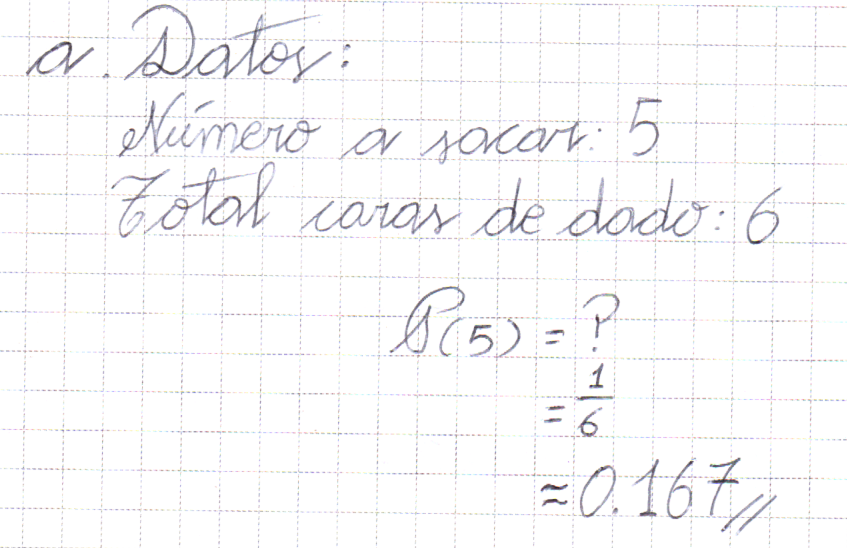
\includegraphics[width=0.97\linewidth]{/pregunta_1/1_a.png}
		\end{figure}
	\item Tuviste suerte y conseguiste la estrella. Ahora, otra vez es tu turno y debes lanzar tres dados seguidos. Necesitas sacar un 6 en cada uno de esos tres lanzamientos para ganar la siguiente estrella. ¿Cuál es la probabilidad de que obtengas tres 6 seguidos?
		\begin{figure}[H]
		\centering
		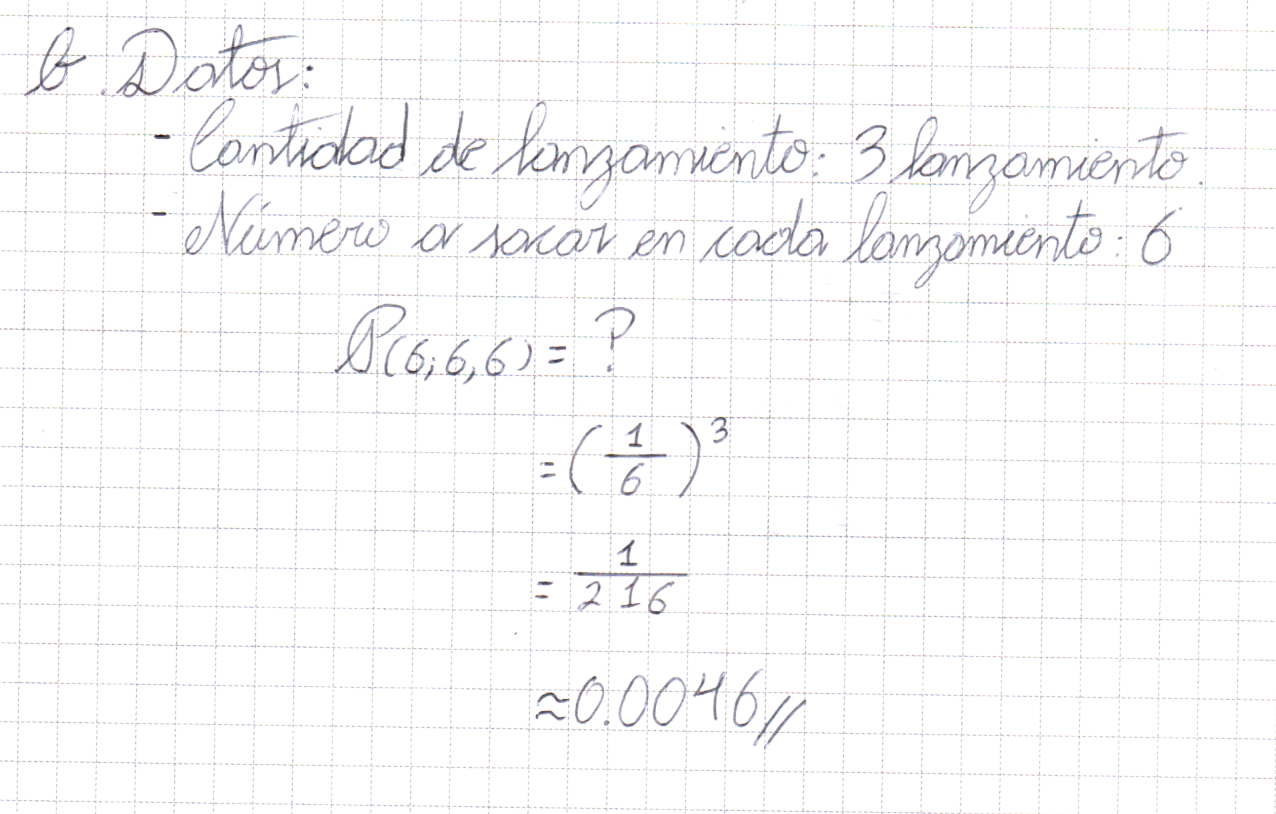
\includegraphics[width=0.64\linewidth]{/pregunta_1/1_b.png}
		\end{figure}
	\item Es el turno de tu amigo, quien lanzará dos dados. Si la suma de ambos dados es 7, él caerá en la casilla del Rey Boo y te robará una estrella. No quieres que eso suceda. ¿Cuál es la probabilidad de que la suma de los dos dados sea 7?
		\begin{figure}[H]
		\centering
		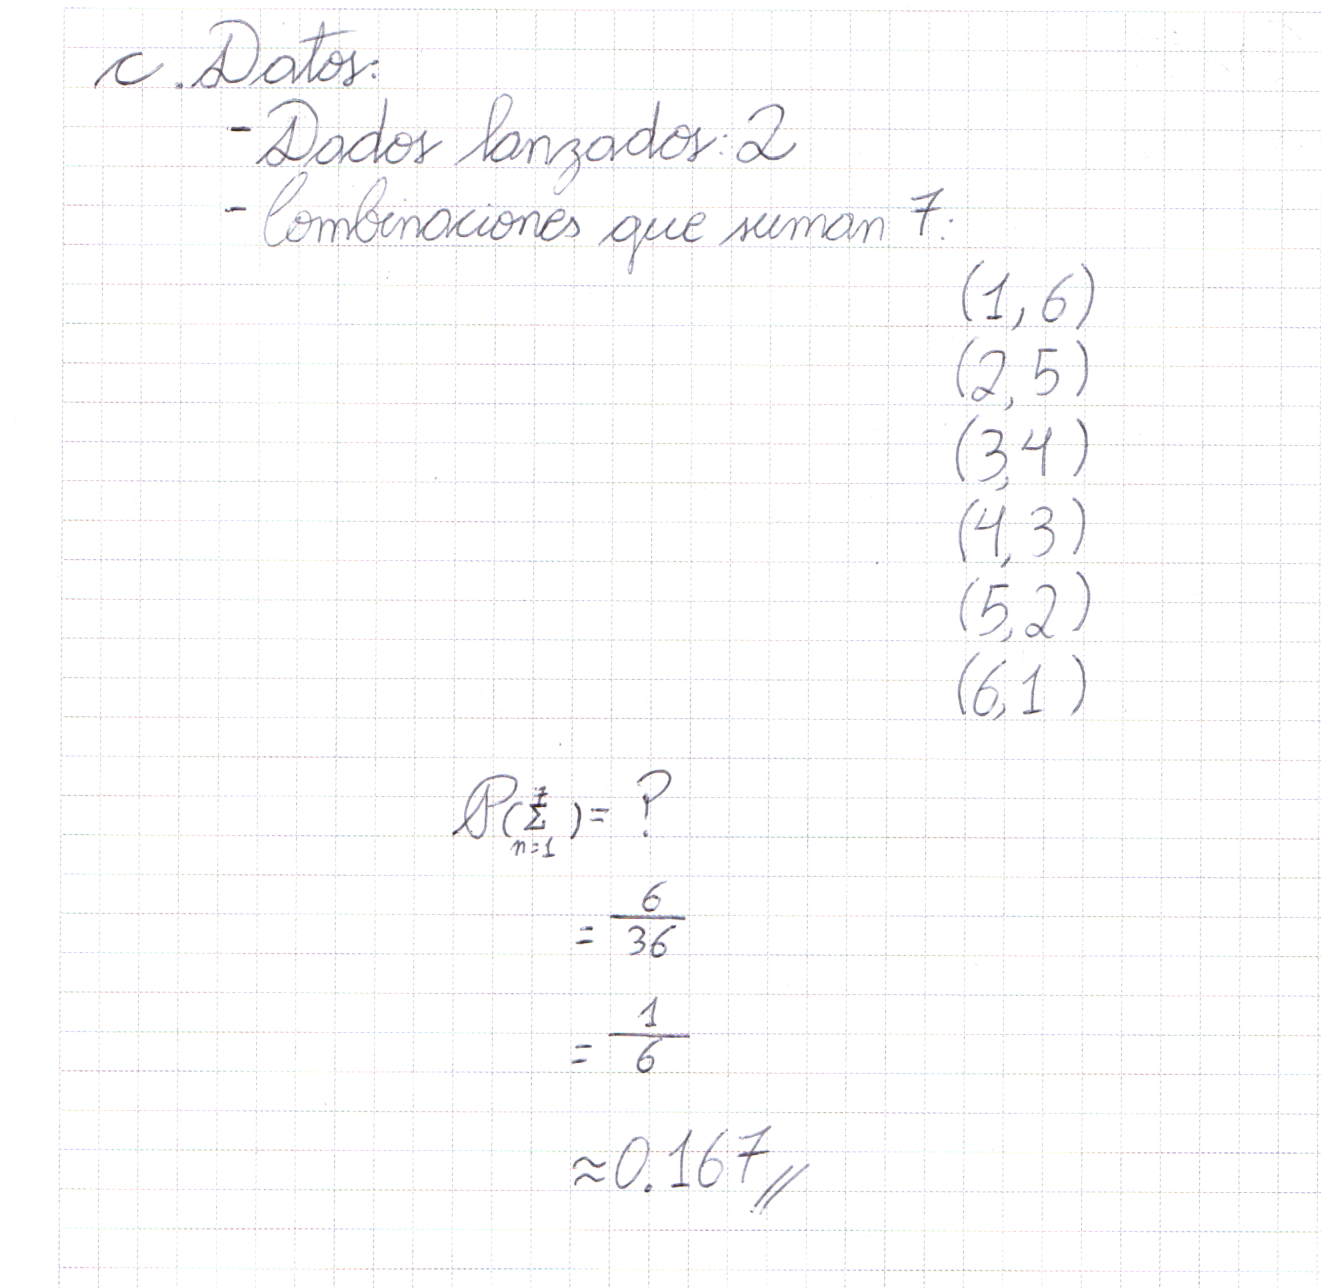
\includegraphics[width=0.64\linewidth]{/pregunta_1/1_c.png}
		\end{figure}
	\item Tu amigo no logra robarte la estrella. Vas ganando el juego y es el último turno. Debes lanzar cuatro dados y evitar parar por el castillo de Bowser. Si caes en el castillo, te robará todas tus estrellas y perderás el juego. Necesitas obtener resultados muy altos para evitar el castillo. Estás preocupado.
	\begin{enumerate}[label=\roman*.]
		\item ¿Cuál es la probabilidad de que, en esos cuatro lanzamientos, obtengas exactamente dos 6? \textbf{Pista:} debes usar una de las funciones de probabilidad que aprendimos en clases.
		\begin{figure}[H]
			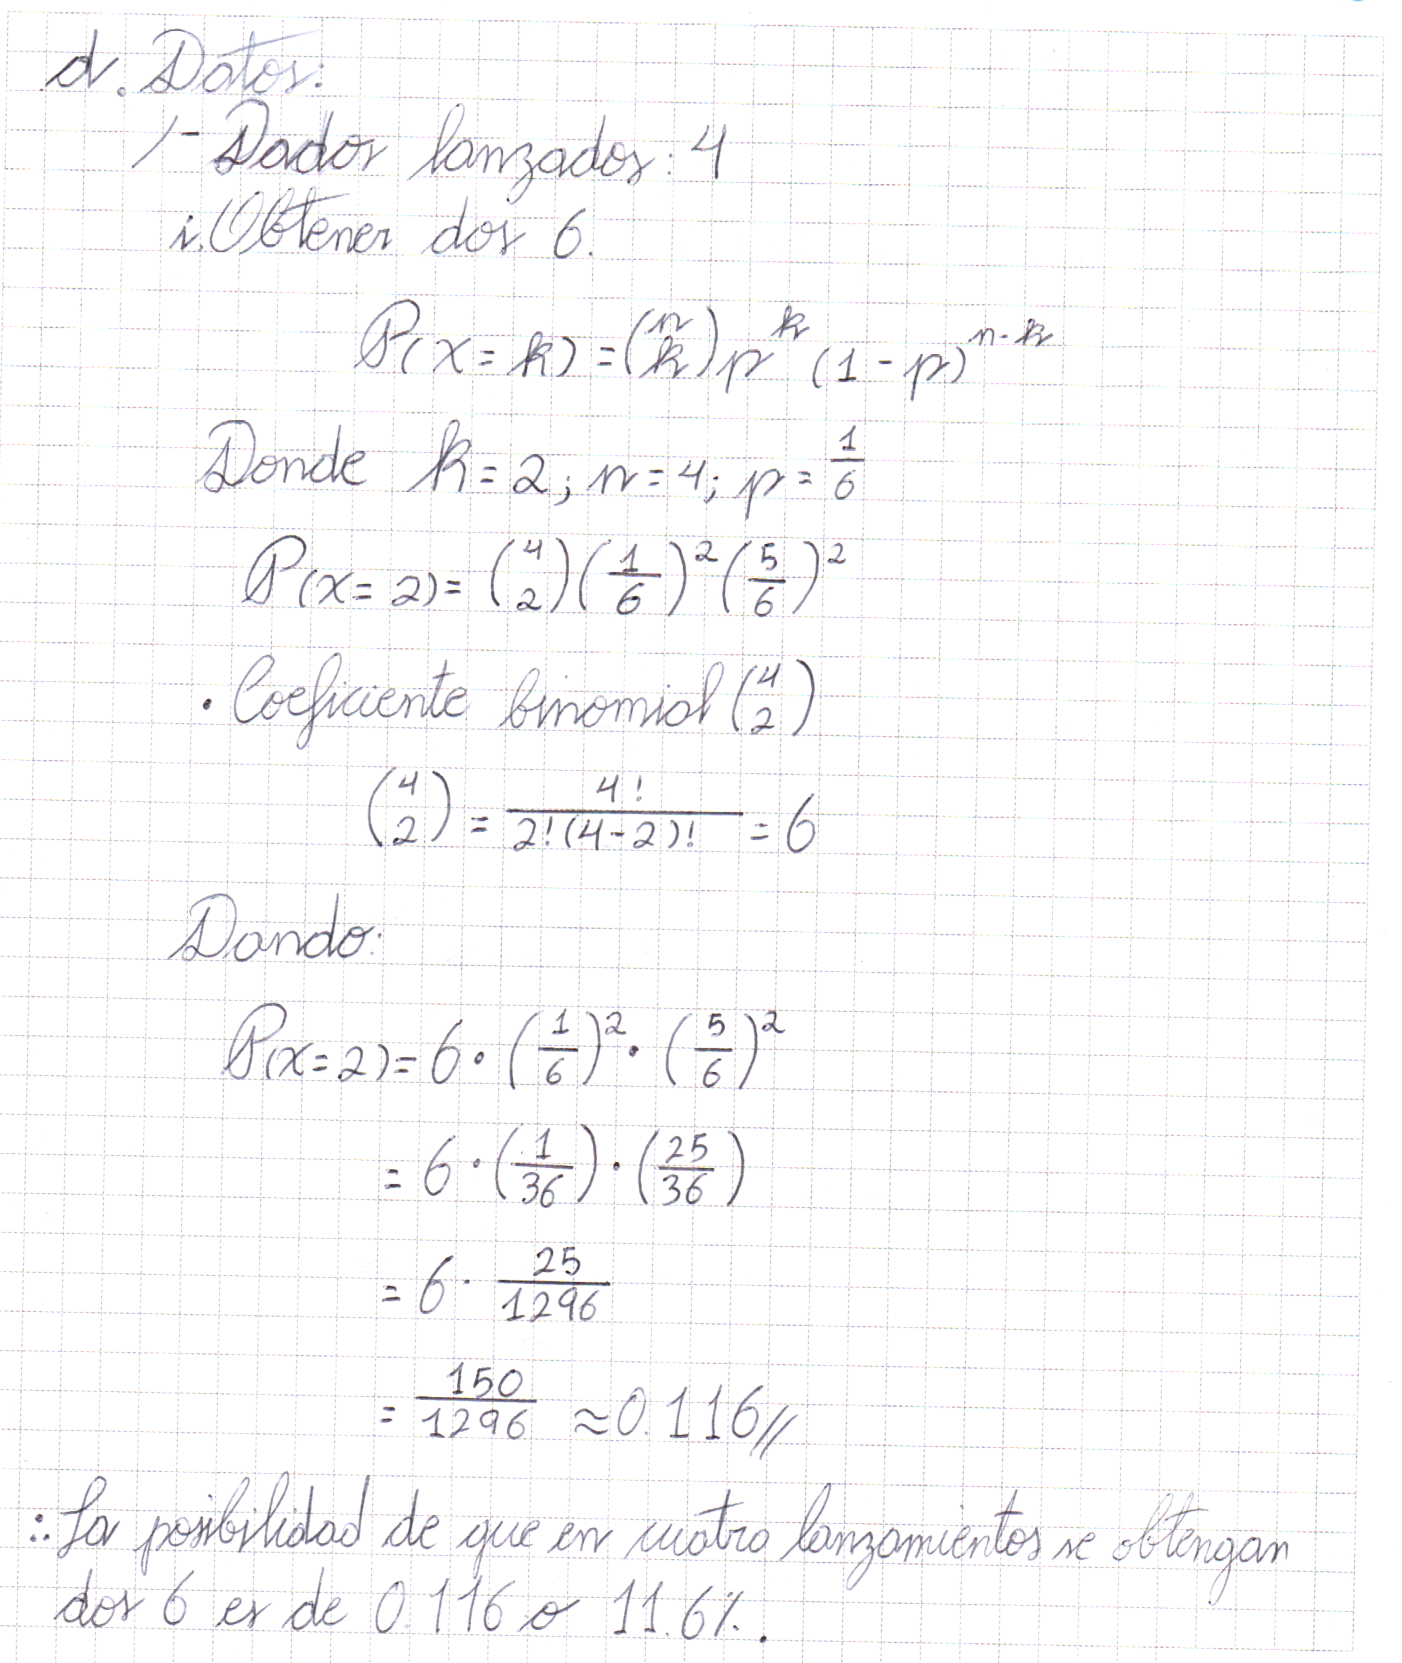
\includegraphics[width=0.91\linewidth]{/pregunta_1/1_d_i.png}
		\end{figure}
		\item ¿Cuál es la probabilidad de que en los cuatro lanzamientos saques al menos un dado con el número 6? \textbf{Pista:} podrías usar la complementaria de la probabilidad de no obtener ningún 6.
		\begin{figure}[H]
			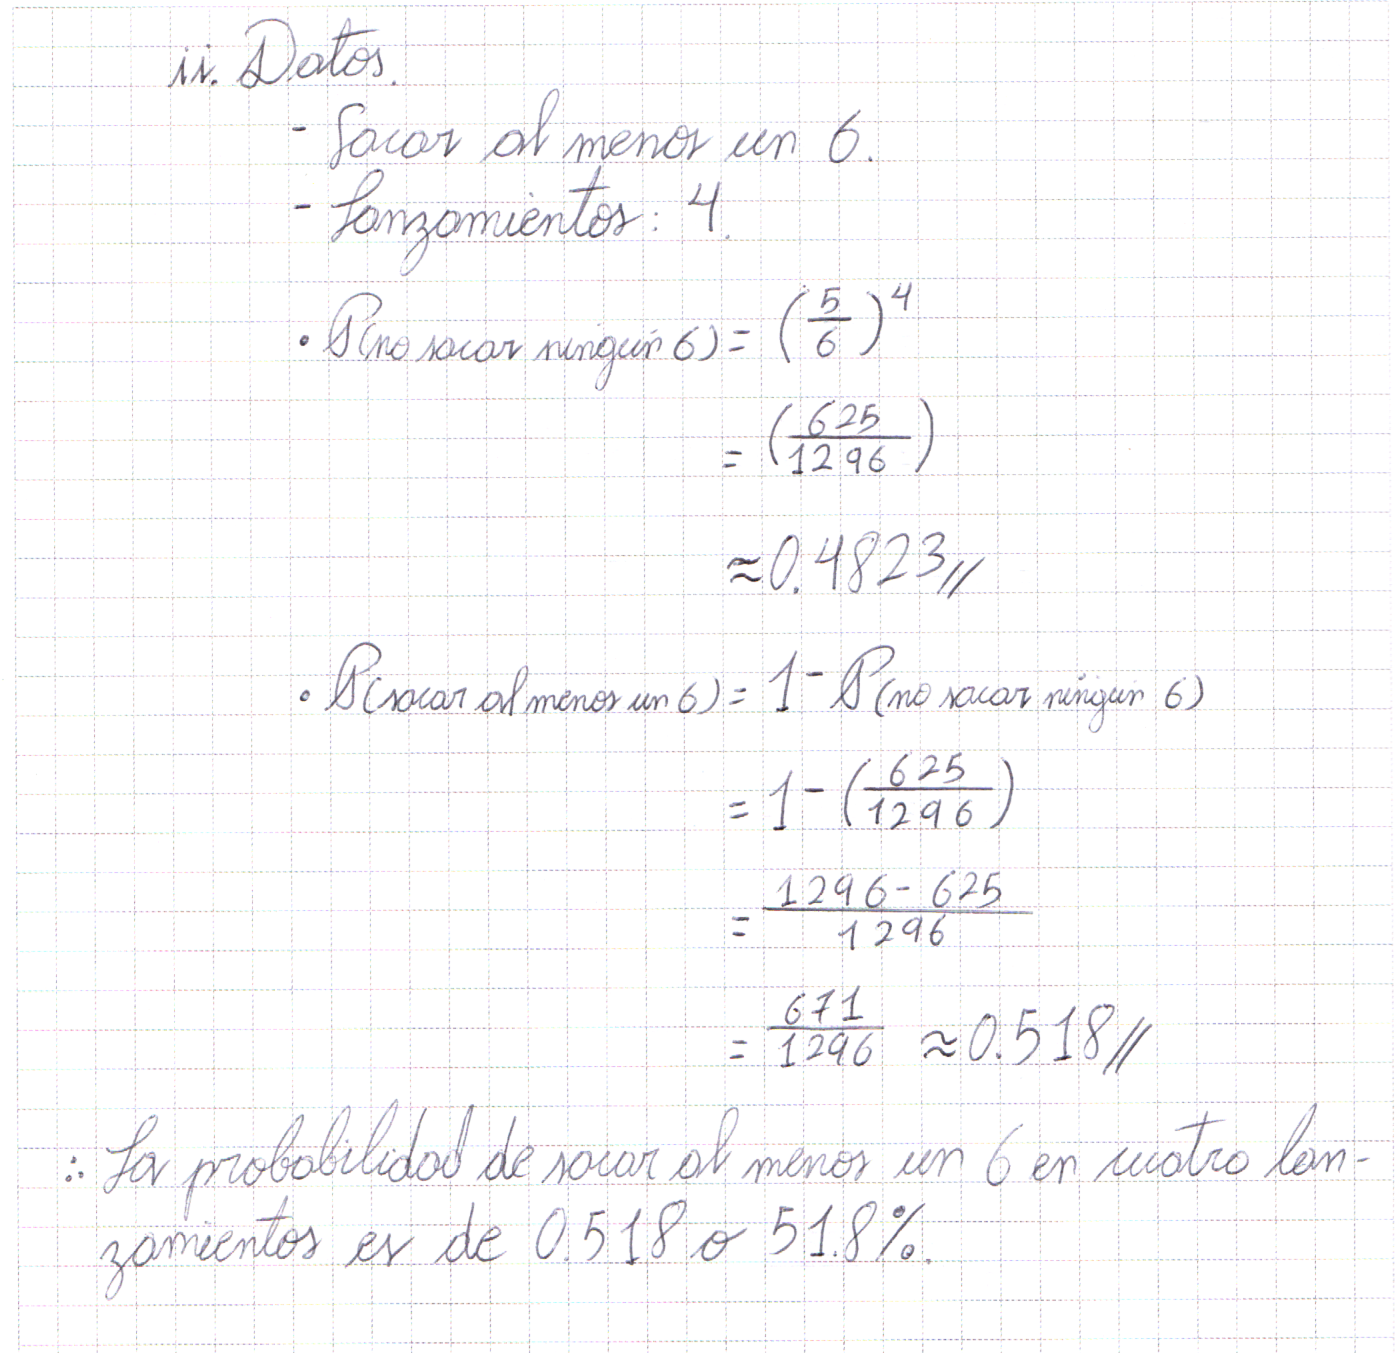
\includegraphics[width=1.12\linewidth]{/pregunta_1/1_d_ii.png}
		\end{figure}
	\end{enumerate}
\end{enumerate}

Tuviste suerte y obtuviste. ¡Estás muy feliz!

\newpage

\section*{Disaster Airlines}

Disaster Airlines ha comenzado a operar en Ecuador, pero ha sido calificada como la peor aerolínea del país.
La empresa ha enfrentado problemas por la sobreventa de vuelos, lo que ha generado numerosas críticas y demandas por parte de los pasajeros.

Tú conoces la mala reputación de Disaster Airlines, pero decides comprar un boleto a la ciudad de Guayaquil porque su precio es más bajo que el de la competencia. Sin embargo, al llegar al aeropuerto, te arrepientes de tu decisión, ya que te informan que tu vuelo ha sido sobrevendido y que no hay espacio para ti. Te ofrecen reubicación en el siguiente vuelo, que sale en cinco horas. ¡Estás furioso!

Pero lo peor aún no termina. La representante de Disaster Airlines se acerca a ti y te informa que en el siguiente vuelo solo hay espacio para cinco pasajeros. Tú eres uno de los 12 pasajeros que esperan abordar
ese mismo vuelo.

\begin{enumerate}[label=\alph*.]
	\item ¿De cuántas formas pueden ser reubicados los 12 pasajeros en los 5 asientos disponibles? Considera que el orden importa, es decir, sentarse en la primera fila es diferente a sentarse en la segunda fila.
		\begin{figure}[H]
		\centering
		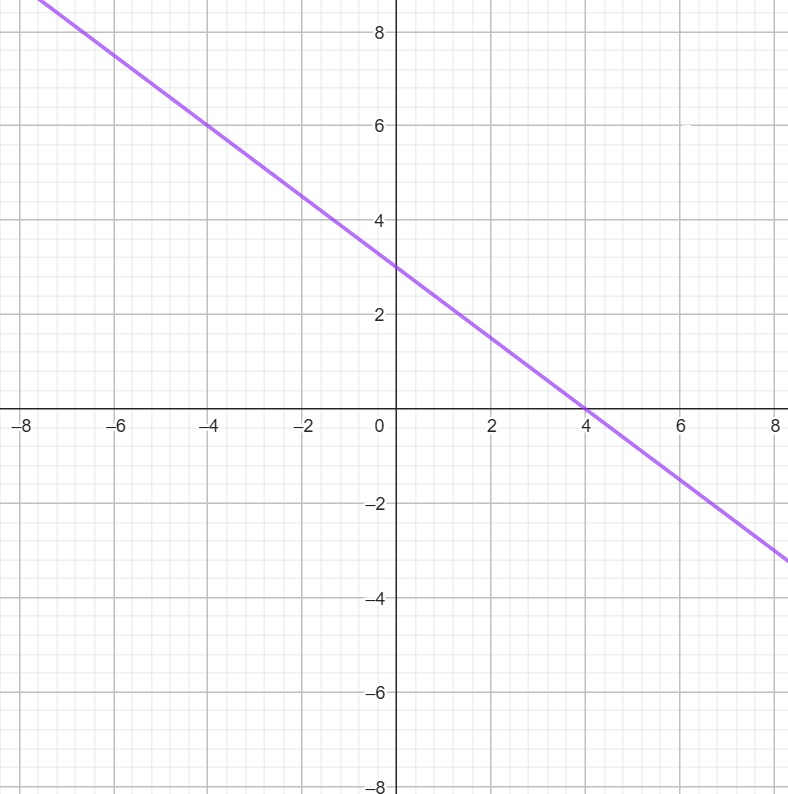
\includegraphics[width=0.88\linewidth]{/pregunta_2/2_a.jpg}
		\end{figure}
	\item Imagina ahora que \textbf{el orden no importa}. Estás tan desesperado por viajar que te da igual en qué asiento te sientes. ¿De cuántas formas pueden ser reubicados los 12 pasajeros en los 5 asientos
	disponibles?
		\begin{figure}[H]
		\centering
		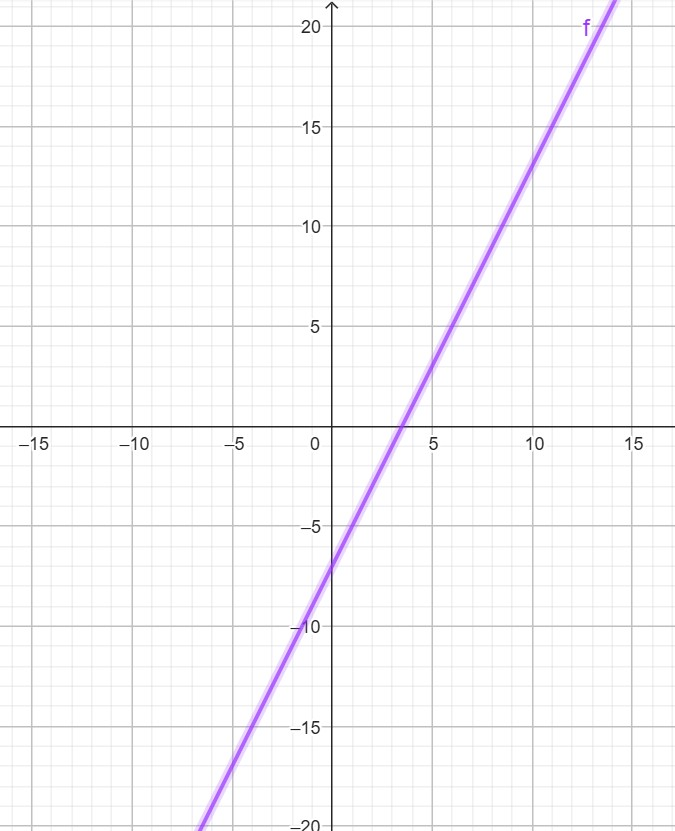
\includegraphics[width=0.71\linewidth]{/pregunta_2/2_b.jpg}
		\end{figure}
	\item ¿Cuál es la probabilidad de que tú seas uno de los cinco pasajeros reubicados en el siguiente vuelo?
	Pista: debes usar una de las funciones de probabilidad que aprendimos en clases.
		\begin{figure}[H]
		\centering
		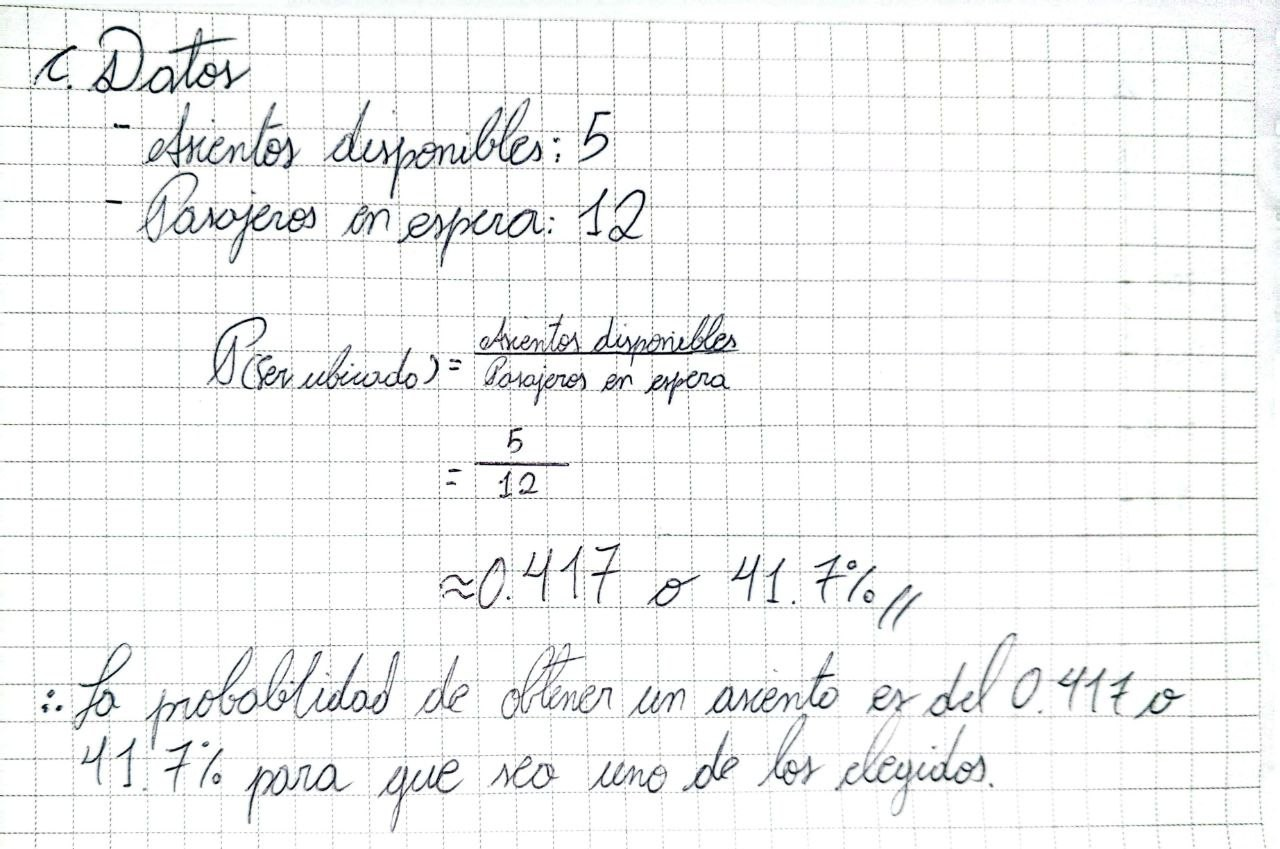
\includegraphics[width=0.79\linewidth]{/pregunta_2/2_c.jpg}
		\end{figure}
\end{enumerate}


\section*{Embarazo adolescente}

Eres una investigadora social y estás preocupada por las altas tasas de embarazo adolescente en Ecuadr. A través de una muestra aleatoria, recolectas datos de una población de 1000 adolescentes. Estos son tus resultados:

\begin{table}[H]
	\centering
	\begin{tabular}{lccc} % Define las columnas (l para alineación izquierda, c para centrado)
		\toprule
		& \textbf{Embarazada Adolescente $A$} & \textbf{No Embarazada $A^c$} & \textbf{Total} \\
		\midrule
		\textbf{Indígena $B$} & 75 & 225 & 300 \\
		\textbf{No indígena $B^c$} & 70 & 630 & 700 \\
		\midrule
		\textbf{Total} & 145 & 855 & 1000 \\
		\bottomrule
	\end{tabular}
	\caption{Distribución de adolescentes por condición y pertenencia indígena.}
	\label{tabla:distribucion}
\end{table}

\begin{enumerate}[label=\alph*.]
	\item Elabora la tabla de probabilidad conjuntas y marginales. Pista: simplemente debes dividir cada celda por el total de la muestra.
	\item ¿Cuál es la probabilidad de que una mujer esté embarazada y sea indígena?
	\item ¿Cuál es la probabilidad de que una mujer esté embarazada y no sea indígena?
	\item ¿Cuál es la probabilidad marginal de que una mujer esté embarazada?
	\item ¿Cuál es la probabilidad marginal de que una mujer sea indígena?
	\item ¿Son eventos independientes el embarazo y la etnia de las adolescentes? Pista: debes comparar la probabilidad conjunta con el producto de las probabilidades marginales.
	\item ¿Cuál es la probabilidad de que una mujer esté embarazada dado que es indígena?
	\item ¿Cuál es la probabilidad de que una mujer sea indígena dado que está embarazada?
\end{enumerate}

\newpage

\section*{La estigmatización de las personas gays}

Uno de los estigmas que más sufren las personas gays es el de ser consideradas como portadoras del VIH. Aunque dentro de la población con VIH el porcentaje de personas gays es alto, no es lo mismo afirmar que una persona con VIH tiene alta probabilidad de ser gay que decir que una persona gay tiene alta probabilidad de tener VIH. Aunque son dos cosas distintas, muchas personas no logran entender la diferencia.

Supongamos que en una población, el 0.1\% de los habitantes tiene VIH. De este grupo, el 60\% son personas gays. Además, se estima que el 5\% de la población total se identifica como gay. Si seleccionamos al azar a una persona gay de esta población, ¿cuál es la probabilidad de que tenga VIH?

\begin{figure}[H]
	\centering
	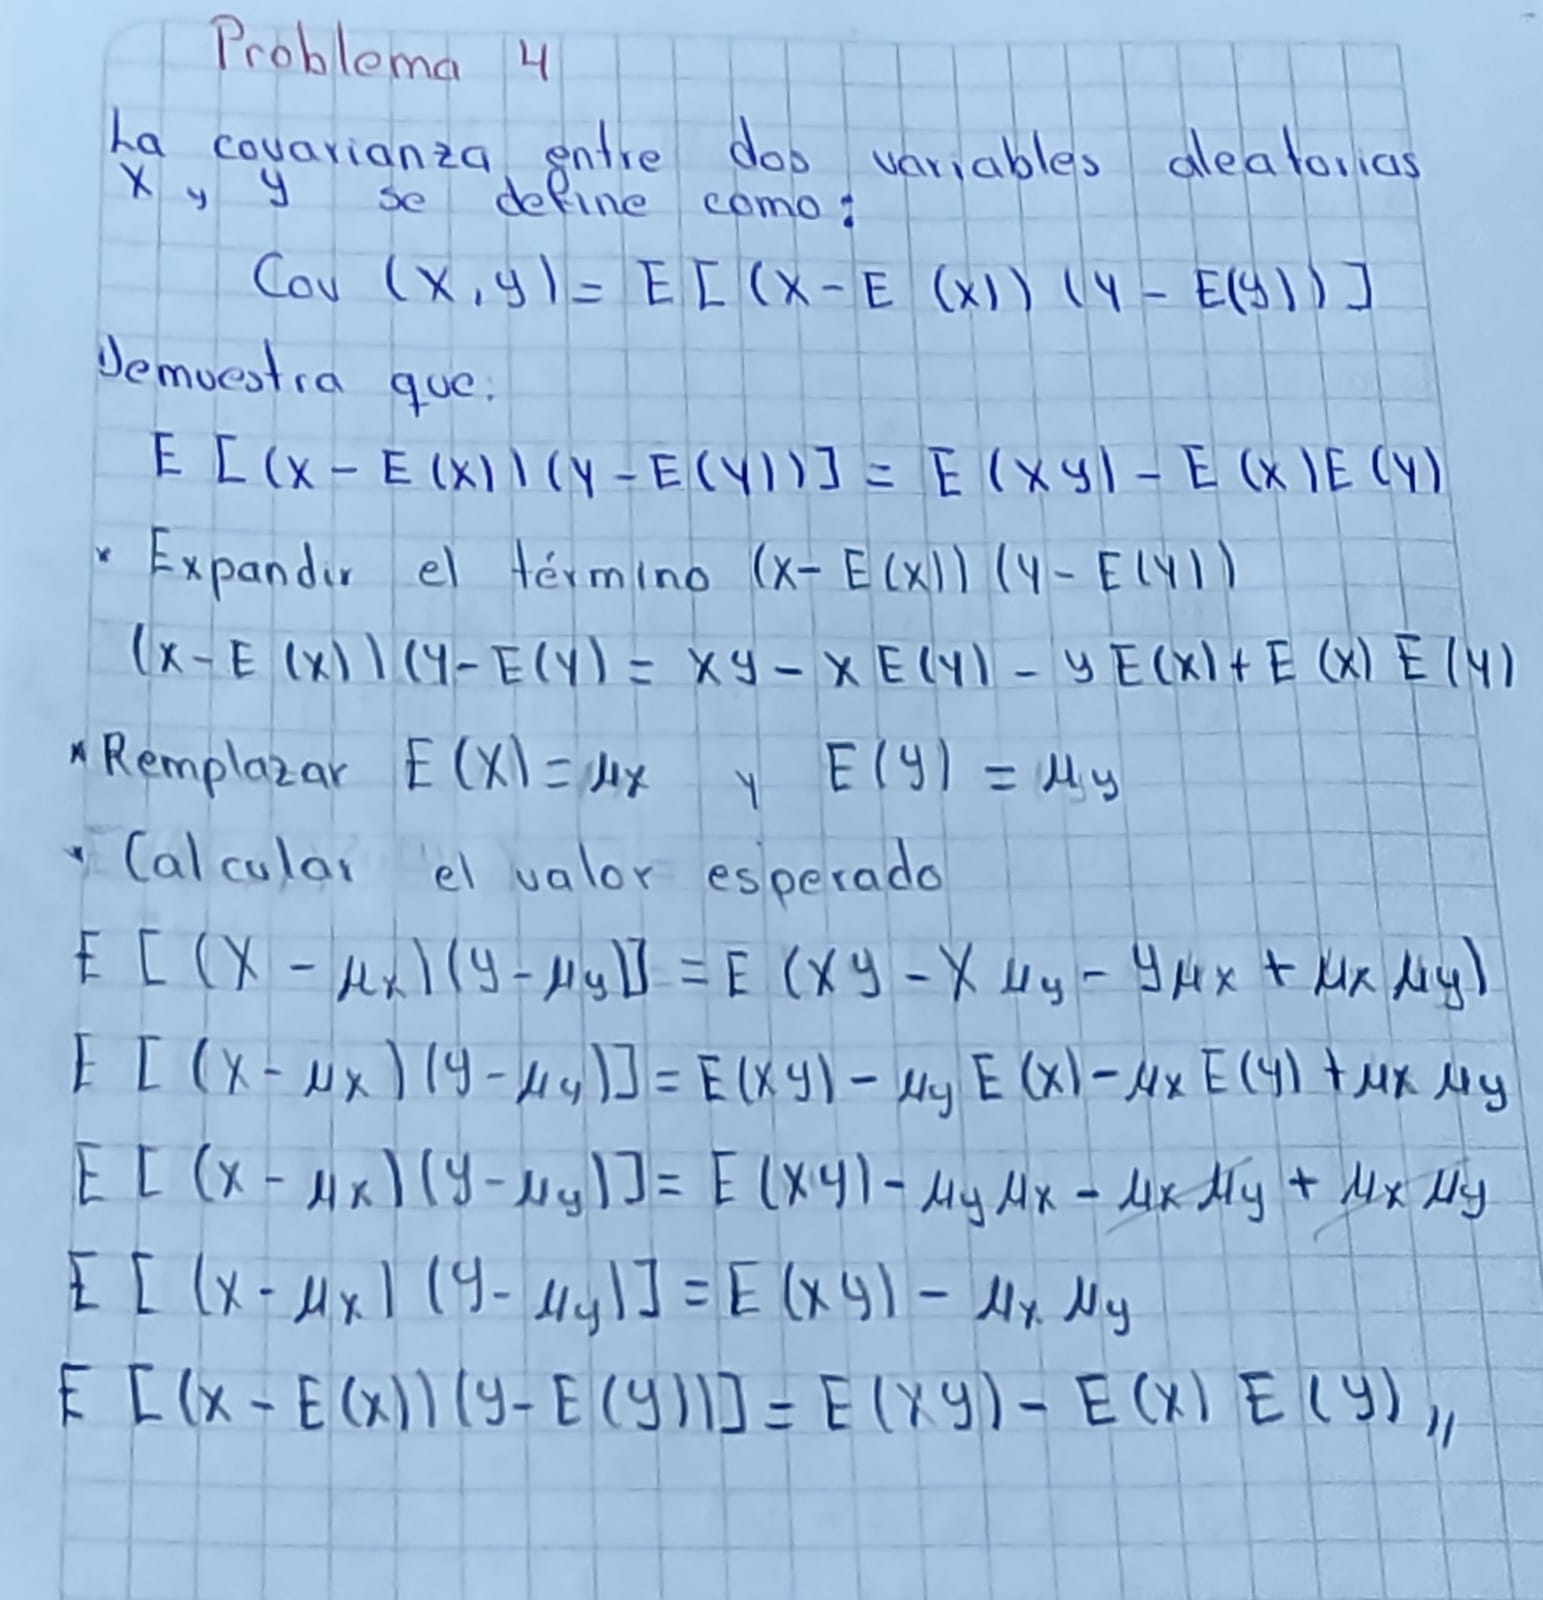
\includegraphics[width=0.89\linewidth]{/pregunta_4/4_a.jpg}
\end{figure}


\section*{El  apocalipsis zombi}

Es el año 2030, y un nuevo patógeno llamado virus Z está comenzando a infectar a la población, transfor-
mando a las personas en zombis. Por fortuna, la prevalencia de la infección aún es baja: solo el 1\% de la población está contagiada. Los científicos de la Universidad Yachay han desarrollado un test para detectar la infección, pero la prueba todavía está en fase experimental y no es muy precisa.

\begin{enumerate}[label=•]
	\item La sensibilidad del test es el 98\%. Es decir, si la persona está infectada con el virus, el test da positivo el 98\% de las veces.
	\item La especificidad del test el del 95\%. Es decir, si la persona no está infectada, el test da negativo el 95\% de las veces.
\end{enumerate}

Vas a la Universidad Yachay y te haces un test... y este da positivo. ¿Cuál es la probabilidad de que realmente estés infectado con el virus Z?

\end{document}
